\documentclass[UTF8,a4paper,12pt]{ctexart}
\usepackage[margin=2.5cm]{geometry}
\usepackage{amsmath,amssymb}
\usepackage{booktabs,array}
\usepackage{graphicx}
\usepackage{caption}
\usepackage{hyperref}

\hypersetup{hidelinks}
\linespread{1.35}
\setlength{\parindent}{2em}
\setlength{\parskip}{0.25em}
\captionsetup{font=small,labelsep=quad}

\title{\bfseries 密立根油滴实验报告\\[0.5em]
\large——平衡法测量电子电量}
\author{姓名：\underline{\hspace{3cm}}\qquad 学号：\underline{\hspace{3cm}}\\[0.5em]
班级：\underline{\hspace{3cm}}}
\date{日期：\underline{\hspace{4cm}}}

\begin{document}

\maketitle

\begin{center}
实验条件：温度 $22\ ^\circ\mathrm{C}$；压强 $1033\ \mathrm{hPa}$；油滴匀速下落距离 $1.60\ \mathrm{mm}$。
\end{center}

\section{实验目的}
\begin{enumerate}
  \item 理解密立根油滴实验的测量原理，掌握用平衡法测量油滴电荷的方法。
  \item 测量基本电荷（电子电量），并根据不同油滴的电荷量分析电荷的量子化特征。
  \item 学习对微小油滴的运动进行 Stokes 修正，以及多次独立测量的数据处理方法。
\end{enumerate}

\section{实验原理}
调节平行板间电压，使带电油滴静止。忽略其他微小作用力，油滴所受电场力与有效重力平衡。考虑空气浮力，有
\begin{equation}
  \frac{qU}{d}=\frac{4}{3}\pi r^3(\rho_{\text{油}}-\rho_{\text{空气}})g,
\end{equation}
式中，$q$ 为油滴电荷量，$U$ 为平衡电压，$d$ 为平行板间距，$r$ 为油滴半径，$g$ 为重力加速度。令 $\rho=\rho_{\text{油}}-\rho_{\text{空气}}$。每一次下落测量分别使用该次记录的下落时间 $t$ 和速度 $v=l/t$，未修正的空气黏滞系数记为 $\eta_0$。

按照参考 PDF 的数据处理方法，由于油滴半径很小，空气不能简单视为连续流体，需要对 Stokes 定律中的黏滞系数作如下修正：
\begin{equation}
  \eta=\frac{\eta_0}{1+\dfrac{b}{pr}},
\end{equation}
其中 $p$ 为空气压强，$b$ 为修正系数。将修正后的黏滞阻力与油滴在空气中的表观重力联立，可直接解得修正后的油滴半径：
\begin{equation}
  r=-\frac{b}{2p}+
  \sqrt{\left(\frac{b}{2p}\right)^2+\frac{9\eta_0 l}{2\rho gt}}.
  \label{eq:radius}
\end{equation}
该式为二次方程的正根，不需要迭代。进一步由平衡条件得到油滴电荷量：
\begin{equation}
  q=\frac{18\pi d}{U\sqrt{2\rho g}}
  \left[\frac{\eta_0 l}{t\left(1+\dfrac{b}{pr}\right)}\right]^{3/2}.
  \label{eq:charge}
\end{equation}
本报告严格采用上述 PDF 方法，每次测量均独立地由式~\eqref{eq:radius} 求修正半径，再由式~\eqref{eq:charge} 求电荷量。取标准电子电量 $e_0=1.602176634\times10^{-19}\ \mathrm{C}$，油滴所带电子数为
\begin{equation}
  n=\operatorname{round}\left(\frac{q}{e_0}\right).
\end{equation}
每次测量给出的电子电量及其相对误差分别为
\begin{equation}
  e_k=\frac{q_k}{n_k},\qquad
  \delta_k=\frac{|e_k-e_0|}{e_0}\times100\%,\qquad k=1,2,\ldots,20.
\end{equation}

\section{实验参数}
\begin{table}[htbp]
  \centering
  \caption{实验参数及计算用常量}
  \begin{tabular}{>{\centering\arraybackslash}p{4.2cm}ccc}
    \toprule
    参数 & 符号 & 数值 & 单位 \\
    \midrule
    温度 & $T$ & $22$ & $^\circ\mathrm{C}$ \\
    空气压强 & $p$ & $1.033\times10^5$ & $\mathrm{Pa}$ \\
    油密度 & $\rho_{\text{油}}$ & $980.0$ & $\mathrm{kg/m^3}$ \\
    空气密度 & $\rho_{\text{空气}}$ & $1.29$ & $\mathrm{kg/m^3}$ \\
    有效密度 & $\rho$ & $978.71$ & $\mathrm{kg/m^3}$ \\
    重力加速度 & $g$ & $9.793$ & $\mathrm{m/s^2}$ \\
    未修正空气黏滞系数 & $\eta_0$ & $1.819412\times10^{-5}$ & $\mathrm{Pa\cdot s}$ \\
    平行板间距 & $d$ & $5.0\times10^{-3}$ & $\mathrm{m}$ \\
    Stokes 修正系数 & $b$ & $8.23\times10^{-3}$ & $\mathrm{N/m}$ \\
    下落距离 & $l$ & $1.6\times10^{-3}$ & $\mathrm{m}$ \\
    \bottomrule
  \end{tabular}
\end{table}

其中油密度和未修正空气黏滞系数由实验给定公式计算：
\begin{align}
  \rho_{\text{油}}&=991-0.5T=980.0\ \mathrm{kg/m^3},\\
  \eta_0&=1.81\times10^{-5}\left[1+0.0026(T-20)\right]
  =1.819412\times10^{-5}\ \mathrm{Pa\cdot s}.
\end{align}

\section{实验步骤}
\begin{enumerate}
  \item 调节仪器，使平行板水平、油滴成像清晰，并熟悉平衡电压调节和计时操作。
  \item 喷入油滴，选择运动缓慢、清晰的带电油滴，调节平衡电压使其稳定悬浮，记录平衡电压 $U$。
  \item 撤去电场，让油滴匀速下落 $1.60\ \mathrm{mm}$，记录下落时间；对同一油滴重复测量两次。
  \item 共测量 10 个油滴，得到 20 次下落时间记录。每次记录分别计算修正半径、电荷量和电子电量，并作 Stokes 修正。
  \item 由每次计算的 $q/e_0$ 确定电子数 $n$，再计算对应的 $e_k$，最后对 20 个独立结果进行统计和线性拟合。
\end{enumerate}

\section{数据记录与处理}
\subsection{原始测量数据}
\begin{table}[htbp]
  \centering
  \caption{10 个油滴的平衡电压和两次下落时间}
  \begin{tabular}{cccc}
    \toprule
    油滴序号 & $U/\mathrm{V}$ & 第 1 次 $t_1/\mathrm{s}$ & 第 2 次 $t_2/\mathrm{s}$ \\
    \midrule
    1  & 89  & 70.49 & 73.01 \\
    2  & 124 & 24.31 & 23.50 \\
    3  & 141 & 25.88 & 26.61 \\
    4  & 158 & 47.94 & 50.48 \\
    5  & 106 & 20.61 & 19.34 \\
    6  & 89  & 28.21 & 27.71 \\
    7  & 211 & 24.51 & 25.11 \\
    8  & 140 & 25.37 & 25.58 \\
    9  & 172 & 21.89 & 23.24 \\
    10 & 85  & 36.81 & 35.88 \\
    \bottomrule
  \end{tabular}
\end{table}

\clearpage
\subsection{Stokes 修正后的独立计算结果}
表中“序号”的前一个数字表示油滴编号，后一个数字表示测量次序。每一次测量均单独代入对应时间，不对两次下落时间作平均。
\begin{table}[htbp]
  \centering
  \caption{20 次测量的油滴半径、电荷量及电子电量}
  \small
  \begin{tabular}{cccccc}
    \toprule
    序号 & $r/\mathrm{\mu m}$ & $q/(10^{-19}\ \mathrm{C})$ & $n$ & $e_k/(10^{-19}\ \mathrm{C})$ & 相对误差 \\
    \midrule
    1-1  & 0.402298 & 1.468524 & 1 & 1.468524 & $8.34\%$ \\
    1-2  & 0.394663 & 1.386497 & 1 & 1.386497 & $13.46\%$ \\
    2-1  & 0.711037 & 5.819480 & 4 & 1.454870 & $9.19\%$ \\
    2-2  & 0.723833 & 6.139332 & 4 & 1.534833 & $4.20\%$ \\
    3-1  & 0.687972 & 4.635759 & 3 & 1.545253 & $3.55\%$ \\
    3-2  & 0.677949 & 4.436098 & 3 & 1.478699 & $7.71\%$ \\
    4-1  & 0.495595 & 1.546509 & 1 & 1.546509 & $3.47\%$ \\
    4-2  & 0.482027 & 1.422938 & 1 & 1.422938 & $11.19\%$ \\
    5-1  & 0.775482 & 8.831575 & 6 & 1.471929 & $8.13\%$ \\
    5-2  & 0.801765 & 9.760297 & 6 & 1.626716 & $1.53\%$ \\
    6-1  & 0.657361 & 6.406945 & 4 & 1.601736 & $0.03\%$ \\
    6-2  & 0.663603 & 6.591185 & 4 & 1.647796 & $2.85\%$ \\
    7-1  & 0.707976 & 3.375998 & 2 & 1.687999 & $5.36\%$ \\
    7-2  & 0.699014 & 3.249396 & 2 & 1.624698 & $1.41\%$ \\
    8-1  & 0.695229 & 4.818188 & 3 & 1.606063 & $0.24\%$ \\
    8-2  & 0.692214 & 4.755783 & 3 & 1.585261 & $1.06\%$ \\
    9-1  & 0.751344 & 4.950135 & 3 & 1.650045 & $2.99\%$ \\
    9-2  & 0.728081 & 4.504421 & 3 & 1.501474 & $6.29\%$ \\
    10-1 & 0.570811 & 4.392251 & 3 & 1.464084 & $8.62\%$ \\
    10-2 & 0.578641 & 4.575492 & 3 & 1.525164 & $4.81\%$ \\
    \bottomrule
  \end{tabular}
\end{table}

\subsection{示例计算}
以第 1 个油滴为例，两次测量分别计算。第 1 次测量使用 $t=70.49\ \mathrm{s}$，由式~\eqref{eq:radius} 得
\begin{equation}
  r_{1,1}=-\frac{b}{2p}+
  \sqrt{\left(\frac{b}{2p}\right)^2+\frac{9\eta_0 l}{2\rho g\times70.49}}
  =0.402298\ \mathrm{\mu m}.
\end{equation}
相应的 Stokes 修正因子为
\begin{equation}
  K_{1,1}=1+\frac{b}{pr_{1,1}}=1.198040.
\end{equation}
代入式~\eqref{eq:charge}，得到
\begin{equation}
  q_{1,1}=1.468524\times10^{-19}\ \mathrm{C},\qquad n_{1,1}=1,
\end{equation}
因此
\begin{equation}
  e_{1,1}=1.468524\times10^{-19}\ \mathrm{C},\qquad \delta_{1,1}=8.34\%.
\end{equation}

第 2 次测量单独使用 $t=73.01\ \mathrm{s}$，同理得到
\begin{align}
  r_{1,2}&=0.394663\ \mathrm{\mu m}, & K_{1,2}&=1.201870,\\
  q_{1,2}&=1.386497\times10^{-19}\ \mathrm{C}, & n_{1,2}&=1,\\
  e_{1,2}&=1.386497\times10^{-19}\ \mathrm{C}, & \delta_{1,2}&=13.46\%.
\end{align}
可见两次测量各自给出完整结果，计算过程中没有使用两次时间的平均值。

\section{实验结果与分析}
20 次独立测量给出的电子电量平均值为
\begin{equation}
  \bar{e}=\frac{1}{20}\sum_{k=1}^{20}e_k
  =1.541554\times10^{-19}\ \mathrm{C}.
\end{equation}
与标准值 $e_0$ 相比，平均值的相对误差为
\begin{equation}
  \delta=\frac{|\bar{e}-e_0|}{e_0}\times100\%=3.784\%,
\end{equation}
即测量结果比标准值低约 $3.784\%$。20 个 $e_k$ 的样本标准偏差为 $8.4630\times10^{-21}\ \mathrm{C}$，单次结果范围为 $1.386497\times10^{-19}$～$1.687999\times10^{-19}\ \mathrm{C}$。

各次测量推得的电子数共出现 1、2、3、4、6 五种不同取值。以 $n$ 为整数对电荷量归一化后，各组 $e_k$ 均接近标准电子电量，实验结果支持油滴电荷呈整数倍分布的量子化特征。

\subsection{电荷量与电子数的线性拟合}
若电荷量子化成立，则油滴电荷量应满足 $q=ne$。以 $10^{-19}\ \mathrm{C}$ 为电荷量单位，对 20 组独立计算的 $(n_k,q_k)$ 作带截距的最小二乘线性拟合：
\begin{equation}
  q=an+b,
\end{equation}
其中斜率 $a$ 对应电子电量。拟合得到
\begin{equation}
  q=(1.561456n-0.031027)\times10^{-19}\ \mathrm{C},
  \qquad R^2=0.987977.
\end{equation}
因此
\begin{equation}
  e_{\mathrm{fit}}=1.561456\times10^{-19}\ \mathrm{C},
\end{equation}
其相对标准值的误差为 $2.542\%$。拟合截距仅为 $-0.031027\times10^{-19}\ \mathrm{C}$，接近理论值零；决定系数 $R^2$ 接近 1，说明电荷量与整数电子数之间具有良好的线性关系。拟合斜率与直接平均所得 $\bar e$ 接近，两种数据处理方法相互印证。

\begin{figure}[htbp]
  \centering
  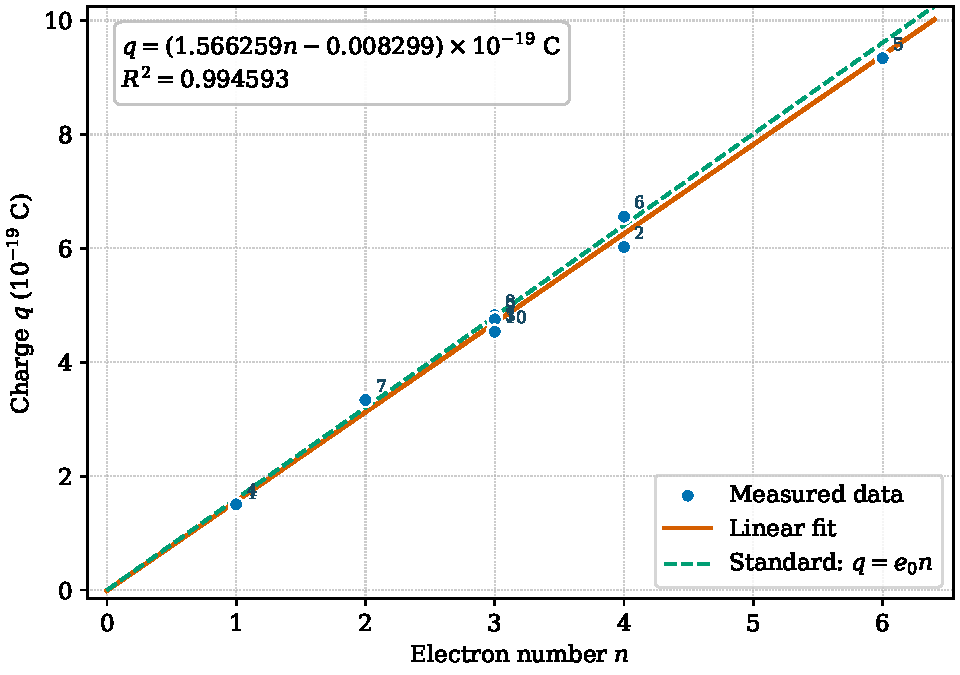
\includegraphics[width=0.88\textwidth]{q_n_fit.pdf}
  \caption{20 次独立测量的电荷量 $q$ 随电子数 $n$ 的关系及线性拟合。橙色实线为拟合结果，绿色虚线为标准关系 $q=e_0n$。}
  \label{fig:qn-fit}
\end{figure}

图~\ref{fig:qn-residual} 给出了各测量点相对于拟合直线的残差。残差分布在零线两侧，未表现出明显的系统性弯曲趋势，说明采用线性关系描述实验数据是合理的。残差的大小反映了计时、平衡电压调节及油滴运动稳定性等因素造成的分散。

\begin{figure}[htbp]
  \centering
  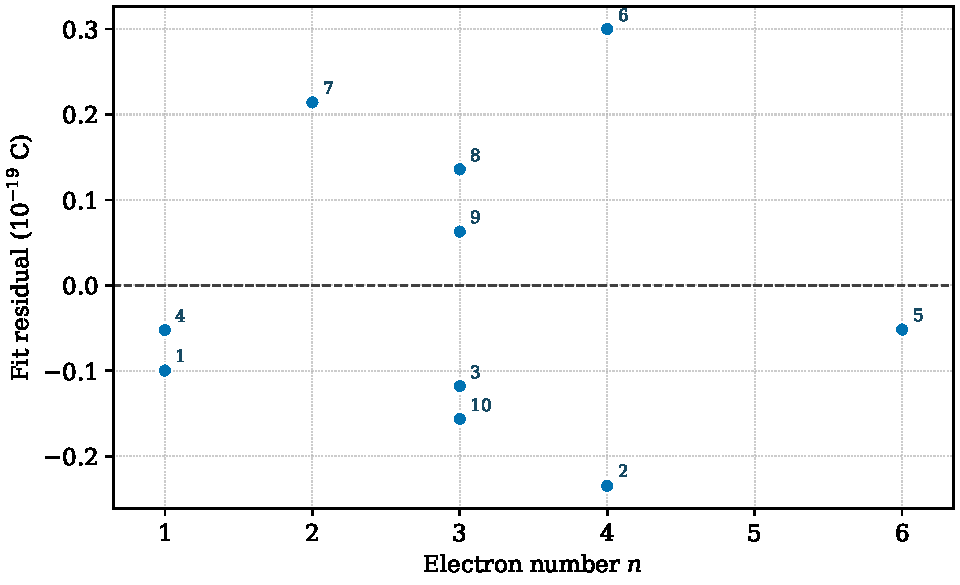
\includegraphics[width=0.88\textwidth]{q_n_residual.pdf}
  \caption{20 次独立计算的电荷量线性拟合残差图，残差单位为 $10^{-19}\ \mathrm{C}$。}
  \label{fig:qn-residual}
\end{figure}

\section{误差分析与注意事项}
\begin{enumerate}
  \item 下落时间由人工计时，启停反应时间以及油滴是否真正达到匀速运动，都会直接影响半径和电荷量。由式~\eqref{eq:radius} 和式~\eqref{eq:charge} 可知，修正半径及电荷量均与本次测量的 $t$ 密切相关，且电荷量对时间的依赖更强，因此计时误差对最终结果尤为敏感。
  \item 油滴若未完全静止，或平衡电压读数存在波动，会使电场力与有效重力不完全平衡。应选择清晰、运动稳定的油滴并细致调压。
  \item 油滴的布朗运动、空气对流、板间距和仪器校准偏差，以及油滴蒸发造成的半径变化，均可能带来系统或随机误差。
  \item Stokes 修正与油滴半径和空气压强有关。本实验统一采用 $T=22\ ^\circ\mathrm{C}$、$p=1033\ \mathrm{hPa}$，严格按照参考 PDF 的解析公式修正半径，未进行迭代求解。
\end{enumerate}

\section{实验结论}
采用平衡法，按照参考 PDF 的方法对每一次测量分别作 Stokes 修正，20 次独立计算得到的电子电量平均值为
\begin{equation}
  \boxed{\bar{e}=1.541554\times10^{-19}\ \mathrm{C}},
\end{equation}
相对标准值的误差为 $3.784\%$。线性拟合给出 $e_{\mathrm{fit}}=1.561456\times10^{-19}\ \mathrm{C}$，且 $R^2=0.987977$。不同油滴的电荷量可分别对应 1、2、3、4、6 个基本电荷，结果与电荷量子化规律相符。

\end{document}
